\documentclass[11pt,a4paper]{article}
\usepackage[utf8]{inputenc}
\usepackage[T1]{fontenc}
\usepackage{xcolor,textcomp,amsmath,amssymb,booktabs,multirow,graphicx,float,hyperref,geometry,array,caption}
\geometry{margin=2.5cm}\emergencystretch=3em
\graphicspath{{figures/}}
\hypersetup{colorlinks=true,linkcolor=blue!50!black,citecolor=blue!50!black,urlcolor=blue!50!black}
\title{AI-Driven Battery Management System for Electric Vehicles:\\ Multi-Stage SOC/SOH Estimation, Fault Diagnosis and Remaining Useful Life Prediction\\[4pt]\large A feasibility-bounded study on CALCE SP20-1 data}
\author{AI-Driven BMS project}
\date{Results generated from the repository state at the time of writing}
\begin{document}
\maketitle
\begin{abstract}
We build a software Battery Management System (BMS) around four experimental files of a single lithium-ion cell (CALCE SP20-1): three 0.1\,A charge/discharge tests labelled 0, 25 and 45\,°C and one 1\,A initial-capacity test. A data audit shows that each file contains one cycle only, that nominal capacity is undocumented, that no temperature channel exists, and that no SOC is measured. Consequently the study is bounded: State-of-Charge (SOC) estimation is evaluated in depth on CALCE, SOH and RUL are guarded pipelines that refuse to output values for CALCE, and fault diagnosis is limited to statistical anomalies plus a clearly labelled simulation benchmark. SOH and RUL are instead evaluated, with leave-one-battery-out validation, on three downloaded ageing datasets whose provenance is kept separate: NASA-style features of seven batteries (provenance unverified), artificial replicas of these, and a PyBaMM simulation. The SOC reference is \emph{calculated} by coulomb integration. Coulomb counting, an Extended Kalman Filter (EKF) on a first-order equivalent-circuit model, Random Forest, gradient boosting, and NumPy LSTM/GRU networks are compared in cross-temperature and cross-rate protocols. With capacity and circuit parameters calibrated at 25\,°C, the EKF achieves a mean absolute error (MAE) of 0.66--1.02 SOC points on the unseen 0\,°C, 45\,°C and 1\,A conditions and recovers from a 30-point initial error, whereas Coulomb counting shows 3.2--6.4 points and does not recover. Tree models are competitive at 0.1\,A (0.4--1.6 points) but fail at 1\,A (13--14 points). We discuss why the per-test normalisation of the reference flatters data-driven models and list all limitations.
\end{abstract}
\tableofcontents
\section{Introduction}
\subsection{Research motivation}
Electric-vehicle battery packs must be operated inside a safe window while delivering maximum range and life. A BMS therefore estimates internal states that cannot be measured directly (SOC, SOH, RUL) and supervises faults \cite{waag2014}. Model-based filters \cite{plett2004ekf1,plett2004ekf2,plett2004ekf3} and data-driven methods \cite{chemali2018,ng2020} compete and complement each other, and their relative merit depends strongly on the data available.

\subsection{Problem statement}
Given four experimental files from one cell, which BMS functions can be developed and validated in a scientifically defensible way, and how do classical and learning-based estimators compare on them? A central part of the problem is to determine --- before modelling --- what the data can \emph{not} support.

\subsection{Research objectives}
(i) Audit the data and fix a valid SOC reference; (ii) compare Coulomb counting, EKF, Random Forest, gradient boosting, LSTM and GRU for SOC, including temperature, rate and noise effects; (iii) implement SOH, RUL and fault-diagnosis modules with explicit feasibility guards; (iv) integrate everything into a BMS engine and dashboard that separates measured, calculated, estimated and simulated quantities; (v) document all limitations.

\subsection{Contributions and scope statement}
The contributions are the audited and reproducible pipeline, the cross-condition SOC benchmark, a gradient-checked NumPy LSTM/GRU, and an explicit demonstration of module infeasibility where data are insufficient. We do \emph{not} claim lifetime prediction, cross-cell generalisation, validation under dynamic drive cycles, or detection of real faults.

\section{Background and literature review}
\subsection{Lithium-ion battery fundamentals}
A lithium-ion cell stores charge in intercalation electrodes; its terminal voltage is the open-circuit voltage (OCV), a monotonic function of SOC at fixed temperature, minus ohmic and polarisation drops that grow at low temperature and high current. Capacity, resistance and OCV depend on temperature and age \cite{waag2014,hu2020joule}. SOC is the fraction of remaining usable charge; SOH is commonly the ratio of present to nominal capacity,
\begin{equation}
\mathrm{SOH}=\frac{Q_{\mathrm{now}}}{Q_{\mathrm{nom}}}\times 100\,\%.
\end{equation}

\subsection{BMS architecture}
Figure~\ref{fig:arch} summarises the implemented architecture: acquisition, preprocessing and feature extraction feed four estimation layers (SOC, SOH, fault diagnosis, RUL), a decision layer produces provenance-tagged reports, and a dashboard exposes them.
\begin{figure}[H]\centering
\fbox{\parbox{0.9\linewidth}{\centering Data files $\rightarrow$ loader (units, de-duplication) $\rightarrow$ segmentation and resampling $\rightarrow$ features\\
$\downarrow$\\
SOC \quad|\quad SOH (guarded) \quad|\quad Fault diagnosis \quad|\quad RUL (guarded)\\
$\downarrow$\\
BMS engine (MEASURED / CALCULATED / ESTIMATED / SIMULATED / UNAVAILABLE) $\rightarrow$ dashboard and reports}}
\caption{Software architecture (see \texttt{docs/SYSTEM\_ARCHITECTURE.md}).}\label{fig:arch}
\end{figure}

\subsection{Related work}
Table~\ref{tab:lit} summarises the publications used. Entries were cited from memory without database access; they must be verified before submission (see \texttt{report/README.md}), and the dataset/limitation columns are intentionally restricted to what is reliably known.
\begin{table}[H]\centering\small
\begin{tabular}{p{2.3cm}p{4.6cm}p{6.6cm}}\toprule
Reference & Method & Relevance here\\\midrule
Plett 2004 \cite{plett2004ekf1,plett2004ekf2,plett2004ekf3} & EKF with equivalent-circuit models for LiPB packs & Basis of our EKF and ECM identification\\
Chemali et al.\ 2018 \cite{chemali2018} & Deep recurrent networks for SOC & Motivates LSTM/GRU baselines\\
Ng et al.\ 2020 \cite{ng2020} & Data-driven ML for SOC and SOH & Motivates tree/ML baselines for SOC and SOH\\
Severson et al.\ 2019 \cite{severson2019} & Cycle-life prediction from early-cycle data & Illustrates the multi-cell, multi-cycle data that SOH/RUL need and our files lack\\
Xing et al.\ 2013, He et al.\ 2011 \cite{xing2013,he2011} & Prognostics on CALCE-type cells & Context for RUL; not reproduced\\
Weng et al.\ 2014 \cite{weng2014} & OCV modelling for SOC/SOH & Context for our pseudo-OCV from a low-rate discharge\\
Waag et al.\ 2014, Hu et al.\ 2020 \cite{waag2014,hu2020joule} & Reviews of monitoring and prognostics & Background on states, temperature effects\\
\bottomrule\end{tabular}
\caption{Literature used.}\label{tab:lit}
\end{table}

\section{CALCE dataset and preprocessing}
\subsection{Dataset description}
Four Excel files of cell SP20-1 were audited (\texttt{docs/DATASET\_AUDIT\_REPORT.md}). Each 0.1\,A test follows: rest (2\,h), constant-current discharge to 2.5\,V, rest (2\,h), constant-current charge, rest. The initial-capacity test uses 1\,A with a constant-voltage phase (Fig.~\ref{fig:raw}). Temperatures 0/25/45\,°C are taken from file names; a single 23\,°C reading exists in the 25\,°C file and the 1\,A file carries no temperature. The files use different schemas (Arbin full export vs.\ reduced export in mV/mA), event-driven vs.\ 1\,s logging, and the 0\,°C file is an OOXML workbook with a \texttt{.xls} extension; the loader is configuration-driven (\texttt{configs/dataset\_config.yaml}).
\begin{figure}[H]\centering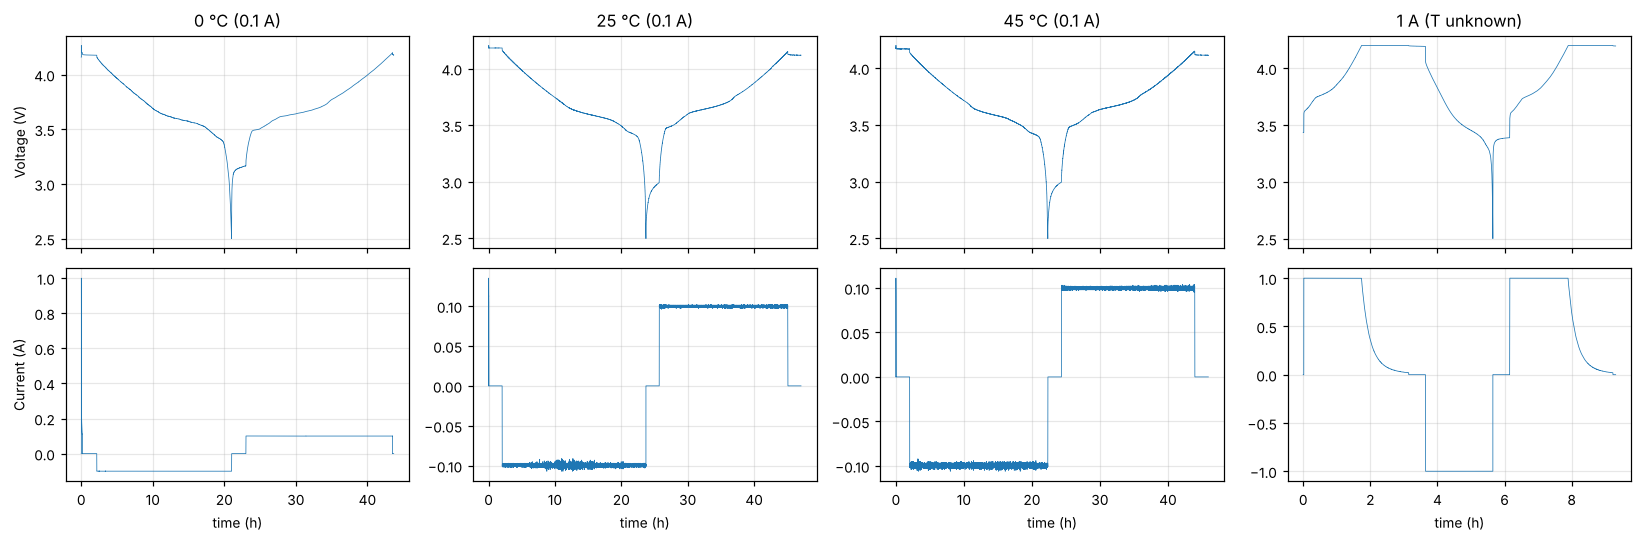
\includegraphics[width=\linewidth]{fig01_raw_overview.png}\caption{Measured voltage and current of the four tests.}\label{fig:raw}\end{figure}
\paragraph{Findings constraining the study.} (1) One cycle per file (no ageing); (2) one cell; (3) no usable temperature measurement; (4) no documented nominal capacity; (5) no measured SOC; (6) 25/45\,°C charge phases stop near 4.15\,V. Table~\ref{tab:capacity} lists measured delivered capacities; the lower value at 45\,°C than at 25\,°C is unexpected and is confounded with test history (tests span Oct.\ 2015--Feb.\ 2016).
\begin{table}[htbp]\centering\footnotesize
\begin{tabular}{lrrrr}
\toprule
 & Mean I (A) & Delivered Q (Ah) & Q / Q$_{25}$ (\%) & R$_0$ ($\Omega$) \\
Condition &  &  &  &  \\
\midrule
0\,°C & -0.100 & 1.882 & 87.240 & 0.132 \\
25\,°C & -0.100 & 2.157 & 100.000 & 0.080 \\
45\,°C & -0.100 & 2.022 & 93.750 & 0.082 \\
1\,A & -1.000 & 2.009 & 93.150 & 0.126 \\
\bottomrule
\end{tabular}
\caption{Measured delivered capacity (2.5\,V cut-off) and R$_0$ at discharge onset per test. Temperatures are file-name labels. These are not SOH values.}\label{tab:capacity}
\end{table}


\subsection{Preprocessing}
The pipeline performs unit conversion, duplicate-timestamp removal, physical-range checks, charge/discharge/rest segmentation from the current sign (20\,mA tolerance, 10\,min minimum), and linear resampling to a 20\,s grid. Features are limited to quantities that exist in all files: voltage, current, a causal 10\,min voltage moving average and a 10\,min voltage difference. Energy, internal-resistance and temperature statistics are not used because they are not available in every file.

\section{Methodology}
\subsection{SOC reference}
Because SOC is not measured, the reference over the main discharge is calculated as
\begin{equation}
\mathrm{SOC}_{\mathrm{ref}}(t)=1-\frac{1}{Q_{\mathrm{dis}}}\int_{t_0}^{t}|I(\tau)|\,\mathrm{d}\tau,\qquad Q_{\mathrm{dis}}=\int_{t_0}^{t_{\mathrm{cut}}}|I|\,\mathrm{d}\tau ,
\end{equation}
with 100\,\% at the start of the discharge and 0\,\% at the 2.5\,V cut-off of that test. It is a calculated, test-normalised quantity affected by current-sensor error; it is never presented as a measured ground truth.

\subsection{SOC estimators}
\paragraph{Coulomb counting.} $\mathrm{SOC}(t)=\mathrm{SOC}_0+\frac{1}{Q_{\mathrm{cal}}}\int I\,\mathrm{d}t$, with $Q_{\mathrm{cal}}=2.157$\,Ah, the delivered capacity of the 25\,°C test. Using each test's own capacity would be circular.
\paragraph{EKF.} A first-order Th\'evenin model, with $i_d>0$ for discharge,
\begin{equation}
V=\mathrm{OCV}(z)-R_0 i_d - V_1,\qquad \dot V_1=-\frac{V_1}{R_1C_1}+\frac{i_d}{C_1},\qquad \dot z=-\frac{i_d}{3600\,Q_{\mathrm{cal}}}
\end{equation}
is discretised and filtered with the EKF state $x=[z,V_1]^\top$ (prediction with $F=\mathrm{diag}(1,e^{-\Delta t/\tau})$, update with $H=[\partial\mathrm{OCV}/\partial z,\,-1]$) \cite{plett2004ekf3}. $R_0$ comes from the rest-to-discharge voltage step, $R_1,\tau$ from a fit of the first 20\,min of discharge, and a pseudo-OCV from the 0.1\,A discharge voltage corrected by $i_d(R_0+R_1)$ \cite{weng2014}. Parameters are constants identified at 25\,°C ($R_0=0.080\,\Omega$, $R_1=0.028\,\Omega$, $\tau=141$\,s).
\paragraph{Data-driven models.} Random Forest \cite{breiman2001} and scikit-learn histogram gradient boosting (not XGBoost \cite{chen2016xgb}, unavailable offline) use the four features; LSTM \cite{hochreiter1997} and GRU \cite{cho2014} (16 units) use 30-step windows of $(V,I)$, are implemented in NumPy with manual back-propagation through time and Adam \cite{kingma2015}, and are validated by finite-difference gradient checks. Scalers are fitted on training data only.

\subsection{SOH and RUL}
SOH uses the definition above only with a verified $Q_{\mathrm{nom}}$. RUL is $\mathrm{RUL}=N_{\mathrm{EOL}}-N$, with $N_{\mathrm{EOL}}$ the first cycle where capacity falls below a threshold fraction of $Q_{\mathrm{nom}}$ (e.g.\ 80\,\%). Both pipelines demand a multi-cycle trajectory, a verified nominal capacity and (RUL) an observed EOL crossing, and otherwise raise \texttt{InsufficientDataError}. Chronological splits are provided for when such data exist.

\subsection{Fault diagnosis}
Window features (60\,s windows, 30\,s hop) are: voltage std., max.\ voltage rate, current std., current deviation from its local set-point, max.\ current step and max.\ sampling gap. A robust $z$-score threshold detector \cite{pedregosa2011}, Isolation Forest \cite{liu2008if} and One-Class SVM \cite{scholkopf2001} are fitted on 0\,°C and 45\,°C windows with thresholds at the 99.5th percentile of training scores; a persistence rule detects a frozen voltage channel. Detections on real data are \emph{statistical anomalies}. A simulator injects five synthetic fault types into the real 25\,°C signal for benchmarking only. A decision layer reports measurement, severity, agreement-based confidence, interpretation, recommended investigation and provenance. Autoencoders and supervised classifiers were not implemented (no labels; data volume not justifying them).

\subsection{Metrics}
$\mathrm{MAE}$, $\mathrm{RMSE}$, $R^2$, maximum absolute error, bias and inference time per 1000 samples; SOC errors are in percentage points.

\section{Experimental setup and validation}
All test conditions are unseen by the fitted models. Protocols: models fitted on 25\,°C and tested on 0\,°C, 45\,°C and 1\,A; two-temperature training with the third temperature held out; all three low-current tests used to predict the 1\,A test (unseen rate). The first 10\,min of each test are excluded for every model so that all are scored on identical samples. Hyper-parameters of tree models are chosen by blocked cross-validation (5 contiguous blocks per training condition, gap equal to the window length) so overlapping samples never straddle the train/validation boundary; recurrent networks use early stopping on a contiguous validation block. Seeds are fixed (42). Noise robustness uses \emph{simulated} perturbations added to the real test signals (Table~\ref{tab:noisedef}). After observing that LSTM/GRU collapse under noise, a variant with a floor on the input standard deviation (\texttt{*\_sf}) was added post hoc; the original variants are kept in every table.
\begin{table}[H]\centering\small
\begin{tabular}{lrrr}\toprule Level & $\sigma_V$ (mV) & $\sigma_I$ (mA) & $I$ bias (mA)\\\midrule low & 5 & 10 & 0\\ medium & 10 & 25 & 0\\ high & 20 & 50 & 0\\ I bias & 0 & 0 & 20\\\bottomrule\end{tabular}
\caption{Simulated perturbation levels.}\label{tab:noisedef}\end{table}
Blocked-CV errors of the tree models (about 7--8 SOC points) are much larger than test errors because each held-out block requires extrapolation along the SOC axis; they serve model selection only.

\section{Results}
\subsection{Physics-based estimators}
Table~\ref{tab:socphys} and Fig.~\ref{fig:traj} show that the EKF stays below 1.1 points MAE on all three unseen conditions, including the 1\,A test, and removes a 30-point initial error within the excluded 10\,min warm-up, whereas Coulomb counting drifts linearly because $Q_{\mathrm{cal}}$ differs from the capacity actually delivered (3.2--6.4 points) and keeps a wrong initial SOC. Identifying parameters on the same test lowers the EKF MAE to about 0.12 points (in-sample, optimistic; see \texttt{docs/EXPERIMENTAL\_RESULTS.md}).
\begin{table}[htbp]\centering\footnotesize
\begin{tabular}{llrrrr}
\toprule
 &  & MAE & RMSE & R$^2$ & MaxAE \\
Test & Estimator &  &  &  &  \\
\midrule
\multirow[t]{4}{*}{0\,°C} & CC (SOC$_0$=100\%) & 6.44 & 7.40 & 0.93 & 12.76 \\
 & EKF (SOC$_0$=100\%) & 0.71 & 0.86 & 1.00 & 2.74 \\
 & CC (SOC$_0$=70\%) & 23.56 & 23.85 & 0.31 & 29.89 \\
 & EKF (SOC$_0$=70\%) & 0.71 & 0.86 & 1.00 & 2.74 \\
\cline{1-6}
\multirow[t]{4}{*}{45\,°C} & CC (SOC$_0$=100\%) & 3.15 & 3.62 & 0.98 & 6.24 \\
 & EKF (SOC$_0$=100\%) & 1.02 & 1.13 & 1.00 & 2.22 \\
 & CC (SOC$_0$=70\%) & 26.85 & 26.91 & 0.12 & 29.94 \\
 & EKF (SOC$_0$=70\%) & 1.03 & 1.14 & 1.00 & 2.22 \\
\cline{1-6}
\multirow[t]{4}{*}{1\,A} & CC (SOC$_0$=100\%) & 3.69 & 4.12 & 0.98 & 6.84 \\
 & EKF (SOC$_0$=100\%) & 0.66 & 0.75 & 1.00 & 1.40 \\
 & CC (SOC$_0$=70\%) & 26.31 & 26.37 & 0.02 & 29.45 \\
 & EKF (SOC$_0$=70\%) & 0.69 & 0.77 & 1.00 & 1.38 \\
\cline{1-6}
\bottomrule
\end{tabular}
\caption{Physics-based SOC estimators (capacity and ECM calibrated on the 25\,°C test) on unseen conditions; errors in SOC points, first 10\,min excluded.}\label{tab:socphys}
\end{table}

\begin{figure}[H]\centering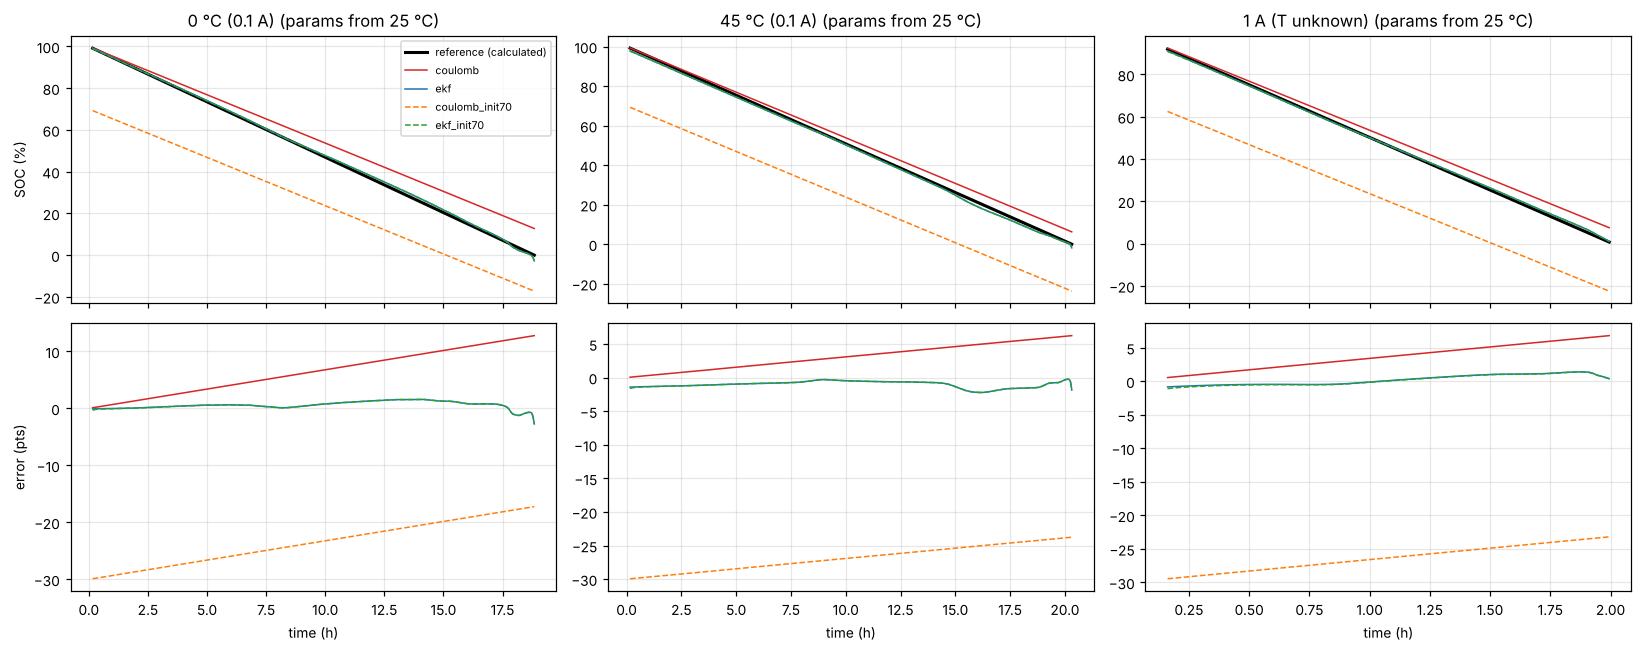
\includegraphics[width=\linewidth]{fig03_physics_soc_trajectories.png}\caption{SOC trajectories and errors of CC and EKF (parameters from 25\,°C) with correct and wrong (70\,\%) initial SOC.}\label{fig:traj}\end{figure}

\subsection{Data-driven estimators and comparative analysis}
Table~\ref{tab:socdd} and Fig.~\ref{fig:dd} give the cross-condition errors. Random Forest and gradient boosting reach 0.4--1.6 points on the 0.1\,A cross-temperature cases and fail on the 1\,A test (13--14 points), because the current lies far outside the training range and the voltage sag is read as lower SOC. The NumPy LSTM/GRU are less accurate and more variable (GRU in particular); their hyper-parameters were not optimised, so no general conclusion on recurrent models is drawn.
\begin{table}[htbp]\centering\footnotesize
\begin{tabular}{lrrrrrr}
\toprule
 & random\_forest & hist\_gradient\_boosting & gru & gru\_sf & lstm & lstm\_sf \\
Train $\rightarrow$ Test &  &  &  &  &  &  \\
\midrule
0\,°C+25\,°C $\rightarrow$ 45\,°C & 1.53 & 1.55 & 9.84 & 6.85 & 1.78 & 1.67 \\
0\,°C+25\,°C+45\,°C $\rightarrow$ 1\,A & 13.20 & 12.96 & 53.46 & 37.63 & 53.01 & 24.37 \\
0\,°C+45\,°C $\rightarrow$ 25\,°C & 1.41 & 1.53 & 11.33 & 9.47 & 1.24 & 1.06 \\
25\,°C $\rightarrow$ 0\,°C & 0.43 & 0.42 & 5.88 & 6.36 & 4.97 & 2.39 \\
25\,°C $\rightarrow$ 1\,A & 13.06 & 14.40 & 29.01 & 101.99 & 42.95 & 41.12 \\
25\,°C $\rightarrow$ 45\,°C & 1.57 & 1.56 & 6.19 & 5.37 & 3.97 & 2.05 \\
25\,°C+45\,°C $\rightarrow$ 0\,°C & 0.75 & 0.69 & 7.06 & 7.51 & 0.92 & 1.04 \\
\bottomrule
\end{tabular}
\caption{Data-driven SOC models: MAE (SOC points) on the unseen test condition (clean signals). \texttt{*\_sf}: std-floor scaling variant added post hoc.}\label{tab:socdd}
\end{table}

\begin{figure}[H]\centering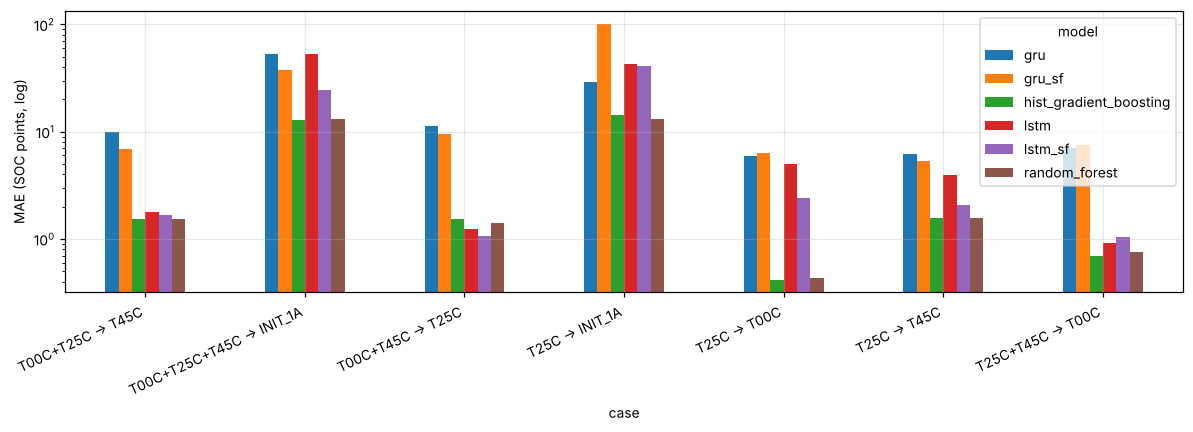
\includegraphics[width=0.85\linewidth]{fig05_data_driven_protocols.png}\caption{MAE of data-driven models per protocol (log scale).}\label{fig:dd}\end{figure}

\subsection{Temperature influence}
Measured delivered capacity at 0.1\,A is 1.882\,Ah at 0\,°C (87\,\% of the 25\,°C value) and $R_0$ at discharge onset is 0.132\,$\Omega$ versus 0.080\,$\Omega$ at 25\,°C (Fig.~\ref{fig:cap}). The EKF and CC, which carry a fixed calibrated capacity, show the corresponding error (CC 6.4 points at 0\,°C). In contrast, data-driven models score well across temperature, but this is largely because each test's reference is normalised by its own capacity, so the capacity change is invisible to the target; the result must not be read as robustness to real capacity variation. Voltage versus reference SOC is nearly temperature-independent at 0.1\,A (Fig.~\ref{fig:vsoc}).
\begin{figure}[H]\centering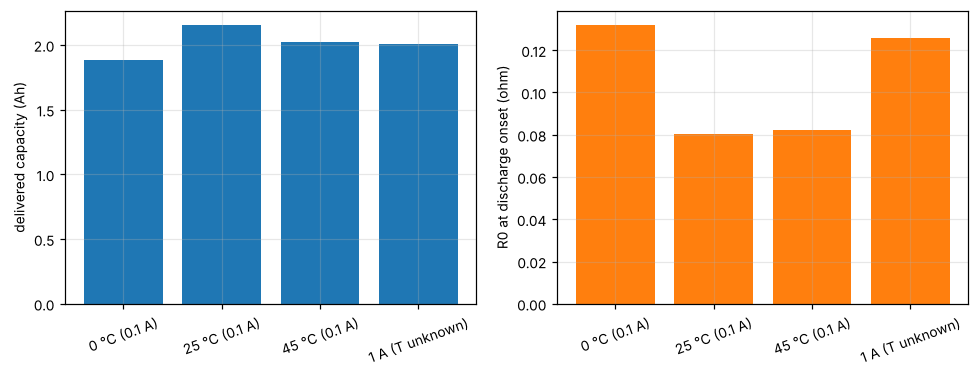
\includegraphics[width=\linewidth]{fig07_capacity_and_r0.png}\caption{Delivered capacity and $R_0$ per condition (labels, not measured temperatures).}\label{fig:cap}\end{figure}
\begin{figure}[H]\centering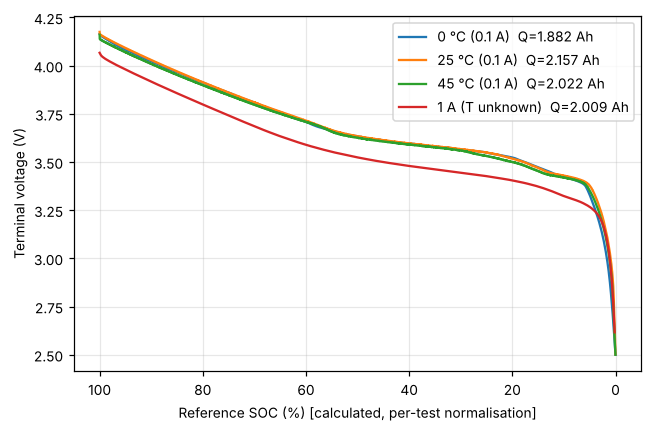
\includegraphics[width=0.6\linewidth]{fig02_voltage_vs_soc_ref.png}\caption{Voltage versus calculated reference SOC.}\label{fig:vsoc}\end{figure}

\subsection{Noise robustness and computational cost}
Table~\ref{tab:noise} (Fig.~\ref{fig:noise}): the EKF is insensitive to noise at its fixed covariance (0.9 points mean MAE), but a 20\,mA current bias raises Coulomb counting to 14 points. Trees degrade gently; the original LSTM/GRU collapse (tens of points) because standardising a nearly constant current (standard deviation of only 0.1--1.6\,mA on the 20\,s grid in the three low-current tests) amplifies noise, which the \texttt{*\_sf} variants remove. Inference costs are in Table~\ref{tab:timing}; all are far below real-time limits at 20\,s sampling.
\begin{table}[htbp]\centering\footnotesize
\begin{tabular}{lrrrrr}
\toprule
 & clean & low & medium & high & I bias 20\,mA \\
\midrule
coulomb & 4.79 & 4.78 & 4.77 & 4.75 & 13.95 \\
ekf & 0.87 & 0.86 & 0.86 & 0.85 & 1.19 \\
random\_forest & 1.00 & 1.01 & 1.05 & 1.16 & 1.00 \\
hist\_gradient\_boosting & 0.99 & 1.05 & 1.20 & 1.66 & 0.98 \\
gru & 6.03 & 60.64 & 70.63 & 70.64 & 25.35 \\
gru\_sf & 5.87 & 5.91 & 6.26 & 7.43 & 8.48 \\
lstm & 4.47 & 18.99 & 22.34 & 28.15 & 24.89 \\
lstm\_sf & 2.22 & 2.27 & 2.41 & 2.89 & 3.43 \\
\bottomrule
\end{tabular}
\caption{Noise robustness with \emph{simulated} perturbations (Table~\ref{tab:noisedef}) added to the real test signals: mean MAE (SOC points) over the 0\,°C and 45\,°C tests, models fitted on 25\,°C.}\label{tab:noise}
\end{table}

\begin{figure}[H]\centering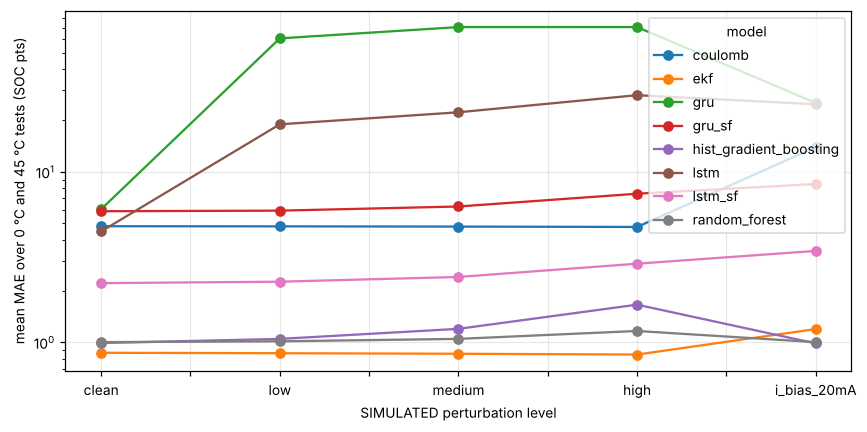
\includegraphics[width=0.75\linewidth]{fig06_noise_robustness.png}\caption{Noise robustness (simulated perturbations).}\label{fig:noise}\end{figure}
\begin{table}[htbp]\centering\footnotesize
\begin{tabular}{lr}
\toprule
 & ms per 1000 samples \\
\midrule
coulomb & 0.02 \\
coulomb\_init70 & 0.02 \\
ekf & 46.93 \\
ekf\_init70 & 46.96 \\
ekf\_matched & 48.33 \\
gru & 14.53 \\
gru\_sf & 14.13 \\
hist\_gradient\_boosting & 4.48 \\
lstm & 21.42 \\
lstm\_sf & 21.32 \\
random\_forest & 11.54 \\
\bottomrule
\end{tabular}
\caption{Mean inference time (NumPy/scikit-learn/Python, single CPU core). The EKF figure is a plain Python loop.}\label{tab:timing}
\end{table}


\subsection{SOH and RUL}
SOH(\%) is not computed: nominal capacity is unverified and one cycle per file gives no degradation trajectory. RUL is not defined for the same reasons (\texttt{results/experiment\_logs/soh\_rul\_feasibility.json}). The delivered-capacity ratios of Table~\ref{tab:capacity} mix temperature, rate and history and are not SOH.

\subsection{Fault diagnosis}
On real data the detectors flag few windows (Table~\ref{tab:faultreal}); of the 80 top-ranked windows (20 per dataset), 50 lie within two minutes of a protocol step transition and are labelled as probable operational events by the decision layer; the remaining 30 are unexplained statistical anomalies. None constitutes evidence of a real fault. The persistence rule fires on constant-voltage charge phases, which are expected. On \emph{simulated} faults (Tables~\ref{tab:faultsim10}, \ref{tab:faultsim05}) the combined detector finds every event at magnitude $\times$1 and $\times$0.5, with different detectors responsible for different fault types; at magnitude $\times$0.25 the extra-resistance fault is missed. Window precision of the combined detector is low (0.24--0.55 at $\times$1), because detectors also flag genuine transitions.
\begin{table}[htbp]\centering\footnotesize
\begin{tabular}{lrrrrrr}
\toprule
 & windows & IF & OC-SVM & Thr. & Flat. & Any \\
\midrule
0\,°C & 5239 & 33 & 37 & 45 & 37 & 96 \\
25\,°C & 5646 & 31 & 33 & 10 & 0 & 39 \\
45\,°C & 5511 & 21 & 17 & 9 & 0 & 25 \\
1\,A & 1116 & 20 & 221 & 44 & 75 & 245 \\
\bottomrule
\end{tabular}
\caption{Windows flagged on the \emph{real} data (statistical anomalies, not validated faults); detectors fitted on 0\,°C and 45\,°C windows.}\label{tab:faultreal}
\end{table}

\begin{table}[htbp]\centering\footnotesize
\begin{tabular}{lrrrrr}
\toprule
 & IF & OC-SVM & Threshold & Flatline & Any \\
\midrule
current\_sensor\_offset & 1.00 & 1.00 & 1.00 & 0.00 & 1.00 \\
resistance\_increase & 1.00 & 1.00 & 0.00 & 0.00 & 1.00 \\
sample\_dropout & 0.25 & 1.00 & 0.00 & 0.00 & 1.00 \\
voltage\_sensor\_stuck & 0.00 & 0.00 & 0.00 & 1.00 & 1.00 \\
voltage\_spike & 1.00 & 1.00 & 1.00 & 0.00 & 1.00 \\
\bottomrule
\end{tabular}
\caption{\emph{Simulated} faults (magnitude $\times$1.0) injected into the real 25\,°C signals: event detection rate (4 events per fault type).}\label{tab:faultsim10}
\end{table}

\begin{table}[htbp]\centering\footnotesize
\begin{tabular}{lrrrrr}
\toprule
 & IF & OC-SVM & Threshold & Flatline & Any \\
\midrule
current\_sensor\_offset & 1.00 & 1.00 & 1.00 & 0.00 & 1.00 \\
resistance\_increase & 1.00 & 0.00 & 0.00 & 0.00 & 1.00 \\
sample\_dropout & 0.25 & 1.00 & 0.00 & 0.00 & 1.00 \\
voltage\_sensor\_stuck & 0.00 & 0.00 & 0.00 & 1.00 & 1.00 \\
voltage\_spike & 1.00 & 1.00 & 0.00 & 0.00 & 1.00 \\
\bottomrule
\end{tabular}
\caption{\emph{Simulated} faults (magnitude $\times$0.5) injected into the real 25\,°C signals: event detection rate (4 events per fault type).}\label{tab:faultsim05}
\end{table}

\begin{figure}[H]\centering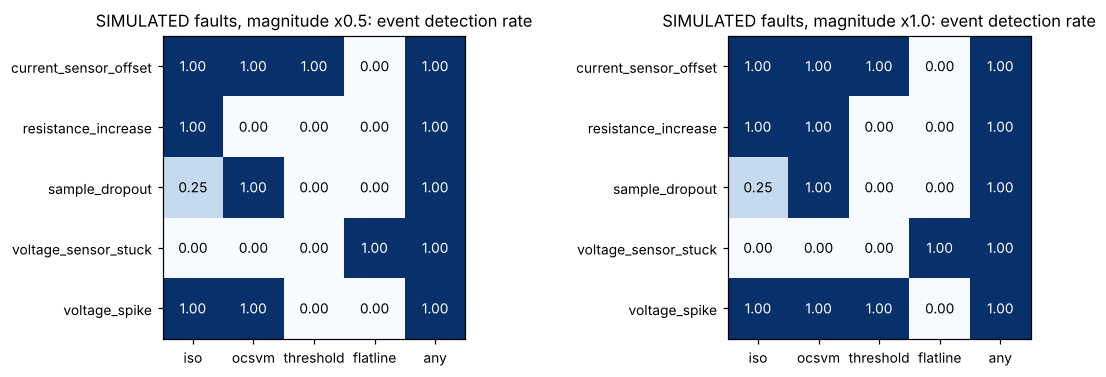
\includegraphics[width=\linewidth]{fig08_fault_simulation_detection.png}\caption{Event detection on \emph{simulated} faults.}\end{figure}

\subsection{Discussion}
The EKF is the most reliable estimator across temperature and rate in this study because its physical structure handles the voltage drop and corrects initial errors; tree models are accurate only inside the training regime; recurrent networks need more data and tuning. All conclusions hold for one cell and constant-current tests.

\section{SOH and RUL on ageing datasets}
\label{sec:aging}
The CALCE files cannot support SOH or RUL (Section~\ref{sec:results}). To exercise these modules, three downloaded CSV files were audited and used. \textbf{Their provenance differs and is kept separate throughout}: (i) \texttt{features\_arrhenius\_tempmean.csv}: battery IDs follow NASA naming and per-cycle features were computed by an unknown third party; we call it ``experimental-derived'' and its provenance is \emph{not verified}; (ii) \texttt{augmented\_full\_dataset.csv}: the same original rows plus three artificial replicas per battery; (iii) \texttt{pybamm\_synthetic\_features.csv}: a PyBaMM \emph{simulation} of six virtual batteries.

\subsection{Audit and definitions}
Table~\ref{tab:agingaudit} shows the rule-based exclusion of two batteries: one holds a single cycle, and one has a capacity reaching 2.6 times its first-cycle value (corrupted trajectory). Seven NASA-style batteries remain (two at 24\,°C, five at 4\,°C; initial capacities 1.08--2.04\,Ah, so no common nominal capacity exists). SOH is therefore defined \emph{relative to the cell's own first-cycle capacity}, $\mathrm{SOH}_{\mathrm{rel}}=Q/Q_1\times100$, \emph{not} to a nominal capacity. The files' own RUL labels were verified to correspond to the first cycle with $Q\le0.70\,Q_1$ (reproduced exactly for all 13 usable batteries), and $\mathrm{RUL}=N_{\mathrm{EOL}}-N$ is expressed in \emph{retained records}: the \texttt{cycle} column indexes retained records whose raw cycle positions are spaced by 2--4. The 70\,\% rule is not the 80\,\% convention mentioned in the project brief; it is the one the data support.
\begin{table}[htbp]\centering\footnotesize
\begin{tabular}{lrrrrr}
\toprule
 & Cycles & Q$_1$ (Ah) & max/first & Ambient (°C) & Usable \\
Battery &  &  &  &  &  \\
\midrule
B0005 & 162 & 1.86 & 1.00 & 24.00 & True \\
B0006 & 102 & 2.04 & 1.00 & 24.00 & True \\
B0033 & 1 & 0.69 & 1.00 & 24.00 & False \\
B0040 & 46 & 0.67 & 2.57 & 24.00 & False \\
B0041 & 22 & 1.22 & 1.00 & 4.00 & True \\
B0045 & 17 & 1.08 & 1.00 & 4.00 & True \\
B0046 & 41 & 1.73 & 1.00 & 4.00 & True \\
B0047 & 41 & 1.67 & 1.00 & 4.00 & True \\
B0048 & 52 & 1.66 & 1.00 & 4.00 & True \\
\bottomrule
\end{tabular}
\caption{Rule-based audit of the NASA-style batteries (exclusion: fewer than 15 cycles, or capacity above 115\,\% of the first cycle).}\label{tab:agingaudit}
\end{table}

\paragraph{Leakage control.} \texttt{RUL}, \texttt{NRUL} and \texttt{battery\_life} are answers; \texttt{capacity\_norm}, \texttt{capacity\_diff} and \texttt{capacity\_ma5} derive from capacity with an unknown normalisation; \texttt{arrhenius\_fade\_rate} is an exact function of \texttt{temp\_mean} ($R^2=1.0000$ in $\log$ rate versus $1/T$). None is used as input (enforced by a guard and unit tests). \texttt{Rct}/\texttt{Re} are constant and back-filled before the first measurement (look-ahead), so they appear only in an exploratory ablation. History features at cycle $k$ use cycles $\le k$ only. The artificial replicas are added only to the training rows of training batteries and never to any test set.

\subsection{Protocols}
Leave-one-battery-out (LOBO): the test battery is never seen in training or in the inner leave-one-battery-out tuning of the Random Forest grid. Temperature transfer: train on the two 24\,°C batteries and test on each 4\,°C battery, and conversely. Ambient temperature labels come from the file. Baselines for RUL: mean training life minus current cycle, and a causal linear extrapolation of $\mathrm{SOH}_{\mathrm{rel}}$ to the 70\,\% level (capped at the longest training life). RUL is evaluated from cycle~5 on.

\subsection{Results on the NASA-style (experimental-derived) data}
\begin{table}[htbp]\centering\footnotesize
\begin{tabular}{lllrrrrr}
\toprule
 &  &  & Batt. & MAE & RMSE & R$^2$ & MaxAE \\
Data & Features & Model &  &  &  &  &  \\
\midrule
\multirow[t]{4}{*}{NASA-style} & \multirow[t]{2}{*}{base} & random\_forest & 7 & 3.38 & 4.13 & 0.80 & 10.24 \\
 &  & linear & 7 & 6.07 & 7.39 & 0.36 & 26.06 \\
\cline{2-8}
 & \multirow[t]{2}{*}{cycle only} & linear & 7 & 8.81 & 10.05 & -0.19 & 18.93 \\
 &  & random\_forest & 7 & 9.00 & 10.45 & -0.29 & 21.45 \\
\cline{1-8} \cline{2-8}
\multirow[t]{4}{*}{PyBaMM (sim.)} & \multirow[t]{2}{*}{cycle only} & linear & 6 & 1.60 & 2.16 & 0.93 & 6.15 \\
 &  & random\_forest & 6 & 1.62 & 2.14 & 0.93 & 6.58 \\
\cline{2-8}
 & \multirow[t]{2}{*}{base} & random\_forest & 6 & 1.89 & 2.35 & 0.92 & 5.62 \\
 &  & linear & 6 & 3.52 & 4.41 & 0.72 & 11.03 \\
\cline{1-8} \cline{2-8}
\bottomrule
\end{tabular}
\caption{SOH leave-one-battery-out, pooled over held-out batteries (SOH points). ``PyBaMM (sim.)'' rows are \emph{simulated} data.}\label{tab:tab_aging_soh}
\end{table}

SOH (Table~\ref{tab:tab_aging_soh}, Fig.~\ref{fig:soh}): Random Forest with the per-cycle signal features reaches a pooled MAE of 3.4 SOH points ($R^2=0.80$), against 6.1 for linear regression; the cycle index alone is inadequate ($R^2<0$) because battery lives range from 17 to 162 records. Features such as incremental-capacity and voltage statistics derive from the same discharge as the capacity, so this is an estimation of capacity from curve features, not an independent validation.
\begin{figure}[H]\centering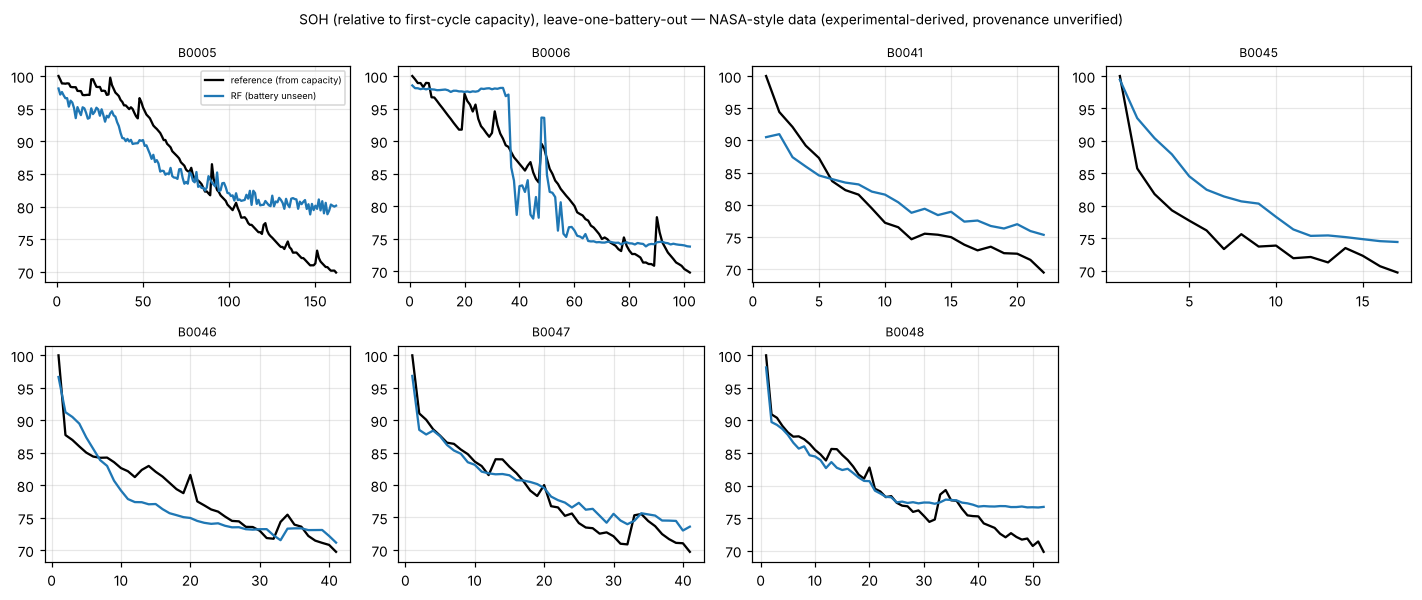
\includegraphics[width=\linewidth]{fig11_aging_soh_nasa_lobo.png}\caption{SOH (relative to first cycle), Random Forest, battery unseen. NASA-style data.}\label{fig:soh}\end{figure}
\begin{table}[htbp]\centering\footnotesize
\begin{tabular}{lllrrrrr}
\toprule
 &  &  & Batt. & MAE & RMSE & R$^2$ & MaxAE \\
Data & Features & Model &  &  &  &  &  \\
\midrule
\multirow[t]{6}{*}{NASA-style} & \multirow[t]{2}{*}{capacity history} & linear & 7 & 17.14 & 23.74 & 0.68 & 76.31 \\
 &  & random\_forest & 7 & 19.90 & 26.79 & 0.59 & 62.37 \\
\cline{2-8}
 & history+signals & random\_forest & 7 & 20.08 & 29.29 & 0.51 & 73.88 \\
\cline{2-8}
 & capacity history & baseline\_linear\_extrap & 7 & 26.20 & 37.38 & 0.20 & 156.00 \\
\cline{2-8}
 & history+signals & linear & 7 & 34.56 & 42.07 & -0.01 & 66.09 \\
\cline{2-8}
 & capacity history & baseline\_mean\_life & 7 & 46.35 & 57.50 & -0.88 & 116.17 \\
\cline{1-8} \cline{2-8}
\multirow[t]{6}{*}{PyBaMM (sim.)} & \multirow[t]{2}{*}{capacity history} & random\_forest & 6 & 7.22 & 10.50 & 0.96 & 46.21 \\
 &  & linear & 6 & 9.11 & 12.72 & 0.95 & 41.17 \\
\cline{2-8}
 & history+signals & random\_forest & 6 & 15.22 & 19.62 & 0.87 & 52.37 \\
\cline{2-8}
 & \multirow[t]{2}{*}{capacity history} & baseline\_linear\_extrap & 6 & 16.13 & 19.82 & 0.87 & 65.77 \\
 &  & baseline\_mean\_life & 6 & 18.40 & 22.74 & 0.83 & 42.00 \\
\cline{2-8}
 & history+signals & linear & 6 & 43.92 & 50.04 & 0.17 & 106.48 \\
\cline{1-8} \cline{2-8}
\bottomrule
\end{tabular}
\caption{RUL leave-one-battery-out, pooled over held-out batteries (records). ``PyBaMM (sim.)'' rows are \emph{simulated} data.}\label{tab:tab_aging_rul}
\end{table}

RUL (Table~\ref{tab:tab_aging_rul}, Fig.~\ref{fig:rulnasa}): the best pooled MAE is 17.1 records (linear regression on capacity-history features, $R^2=0.68$), then Random Forest at 19.9, the linear-extrapolation baseline at 26.2 and the mean-life baseline at 46.4 ($R^2<0$). Adding the signal features \emph{degrades} both models (linear: 34.6). Relative to the battery life the errors are large for the short-lived batteries (per-battery MAE of 6--45\,\% of life for the Random Forest and 12--74\,\% for linear regression). The Random Forest cannot predict beyond the longest training life: with B0005 (162 records) held out, its predictions saturate near 100 (Fig.~\ref{fig:rulnasa}). The 5--95\,\% spread of the trees is a heuristic, not a calibrated interval: it contains the true RUL for only 54\,\% of the points on average (nominal 90\,\%).
\begin{figure}[H]\centering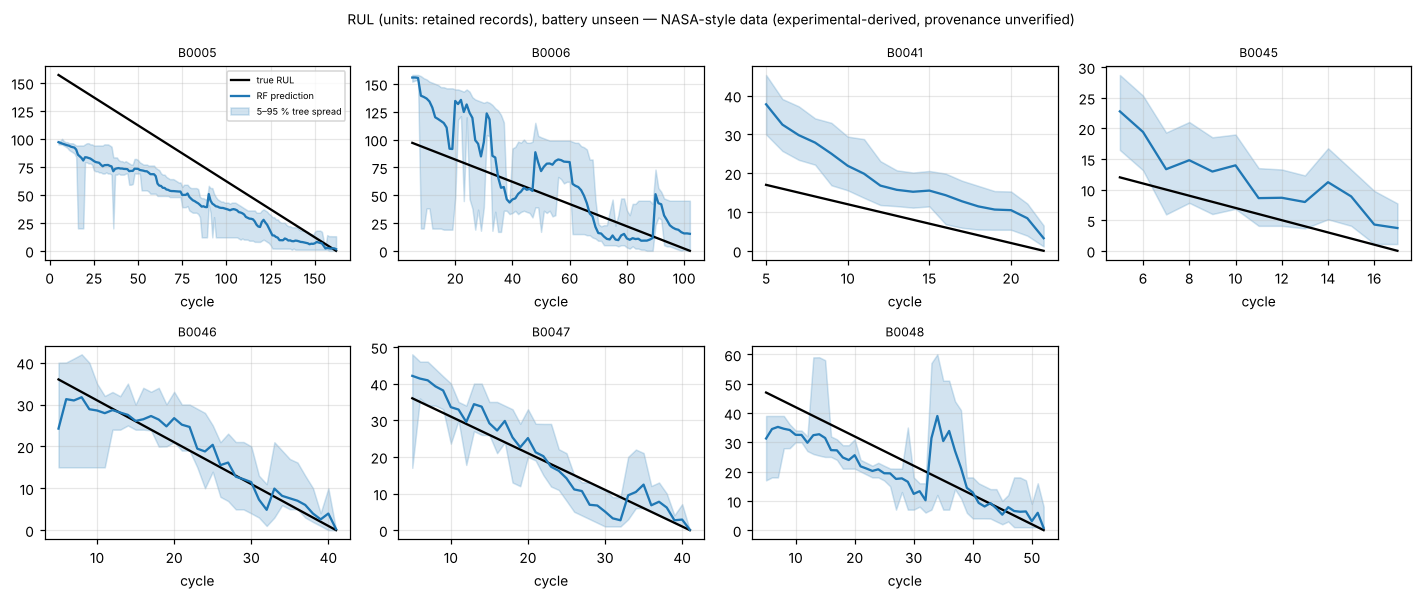
\includegraphics[width=\linewidth]{fig12_aging_rul_nasa_lobo.png}\caption{RUL (retained records), Random Forest on capacity-history features, battery unseen. NASA-style data.}\label{fig:rulnasa}\end{figure}
\begin{table}[htbp]\centering\footnotesize
\begin{tabular}{llllrrrr}
\toprule
 &  &  &  & Batt. & MAE & RMSE & R$^2$ \\
Target & Protocol & Features & Model &  &  &  &  \\
\midrule
\multirow[t]{10}{*}{RUL} & \multirow[t]{4}{*}{cross\_temperature\_24to4} & capacity history & linear & 5 & 12.21 & 14.71 & -0.42 \\
\cline{3-8}
 &  & history+signals & linear & 5 & 26.29 & 30.14 & -4.98 \\
\cline{3-8}
 &  & capacity history & random\_forest & 5 & 19.48 & 21.81 & -2.13 \\
\cline{3-8}
 &  & history+signals & random\_forest & 5 & 12.17 & 13.72 & -0.24 \\
\cline{2-8} \cline{3-8}
 & \multirow[t]{4}{*}{cross\_temperature\_4to24} & capacity history & linear & 2 & 40.79 & 49.65 & -0.37 \\
\cline{3-8}
 &  & history+signals & linear & 2 & 44.16 & 54.51 & -0.65 \\
\cline{3-8}
 &  & capacity history & random\_forest & 2 & 43.99 & 56.19 & -0.75 \\
\cline{3-8}
 &  & history+signals & random\_forest & 2 & 38.03 & 48.84 & -0.32 \\
\cline{2-8} \cline{3-8}
 & \multirow[t]{2}{*}{lobo\_with\_augmented\_training\_rows} & \multirow[t]{2}{*}{history+signals} & linear & 7 & 34.59 & 42.11 & -0.01 \\
 &  &  & random\_forest & 7 & 22.26 & 31.70 & 0.43 \\
\cline{1-8} \cline{2-8} \cline{3-8}
\multirow[t]{6}{*}{SOH} & \multirow[t]{2}{*}{cross\_temperature\_24to4} & \multirow[t]{2}{*}{base} & linear & 5 & 3.79 & 4.99 & 0.47 \\
 &  &  & random\_forest & 5 & 5.50 & 6.73 & 0.03 \\
\cline{2-8} \cline{3-8}
 & \multirow[t]{2}{*}{cross\_temperature\_4to24} & \multirow[t]{2}{*}{base} & linear & 2 & 6.16 & 7.17 & 0.47 \\
 &  &  & random\_forest & 2 & 8.21 & 9.45 & 0.07 \\
\cline{2-8} \cline{3-8}
 & \multirow[t]{2}{*}{lobo\_with\_augmented\_training\_rows} & \multirow[t]{2}{*}{base} & linear & 7 & 6.14 & 7.46 & 0.34 \\
 &  &  & random\_forest & 7 & 3.17 & 3.89 & 0.82 \\
\cline{1-8} \cline{2-8} \cline{3-8}
\bottomrule
\end{tabular}
\caption{NASA-style data: temperature transfer (24\,°C$\leftrightarrow$4\,°C) and augmentation ablation.}\label{tab:agingtransfer}
\end{table}

Temperature transfer and augmentation (Table~\ref{tab:agingtransfer}): no successful cross-temperature generalisation was obtained. $R^2$ never exceeds 0.47 for SOH and is negative for every RUL model; the 24\,°C$\rightarrow$4\,°C direction rests on only two training batteries and the reverse on two test batteries. Adding artificial replicas of the training batteries brings no consistent gain (Random Forest SOH MAE 3.4$\rightarrow$3.2; RUL 20.1$\rightarrow$22.3), consistent with replicas carrying no new information.

\subsection{Results on the simulated PyBaMM data}
\emph{These results are simulated and are not experimental evidence.} Cycle index alone gives $R^2=0.93$ for SOH (MAE 1.6 points) and the signal features do not improve it, which shows that the virtual batteries age in nearly identical ways. Random Forest on capacity-history features reaches an RUL MAE of 7.2 records ($R^2=0.96$) against 16.1 and 18.4 for the baselines. This indicates that the pipeline works on well-behaved data; it says nothing about real batteries.

\subsection{Interpretation and limits}
Seven batteries from two ambient temperatures give low statistical power: pooled metrics are dominated by the longest-lived batteries, and the ranking of models could change with other cells. SOH here is relative to the first cycle, EOL follows the dataset's 70\,\% rule, RUL is in records, and the provenance of the features is unverified. Conclusions are limited to: (i) the pipeline respects leakage and battery-level separation, (ii) on the experimental-derived data, capacity-history features support a moderately accurate RUL and signal features support SOH, (iii) temperature transfer and augmentation were not shown to help.

\section{Limitations}
CALCE: no ageing data, unverified nominal capacity, one cell, no temperature measurement, no measured SOC, constant-current tests only, confounded test history, in-sample EKF identification at 25\,°C, no gradient-boosting library other than scikit-learn's, NumPy recurrent networks of small size without extensive tuning, unverified literature entries and an unexecuted (stub-tested) dashboard. See \texttt{docs/LIMITATIONS.md}.
\section{Future research directions}
Verified-provenance multi-cell ageing data with documented nominal capacity and calibrated RUL uncertainty (e.g.\ conformal intervals); dynamic drive-cycle data (e.g.\ US06/FUDS) to test the SOC methods under realistic loads; temperature-dependent and SOC-dependent ECM parameters and adaptive EKF noise tuning; a measured temperature channel for over-temperature diagnosis; hyper-parameter optimisation of recurrent models with a standard deep-learning framework; protocol-aware anomaly detection.
\section{Conclusion}
Within what four single-cycle files can support, a reproducible BMS pipeline was built and SOC estimation was benchmarked across temperature, rate and noise: the EKF generalised best, trees excelled only at low current, and recurrent networks were not competitive. SOH, RUL and real fault diagnosis were shown to be infeasible on the CALCE files and are therefore guarded rather than faked. On separate ageing data (seven NASA-style batteries of unverified provenance, and a simulation), SOH and RUL were estimated with strict battery-level separation: moderate accuracy for RUL from capacity-history features, no demonstrated temperature transfer, and results on the simulated data that carry no experimental weight.

\bibliographystyle{unsrt}
\bibliography{references}
\appendix
\section{Reproducibility}
Scripts (\texttt{scripts/}) regenerate audit, results, figures and the tables included here. Configuration is in \texttt{configs/}; seeds are fixed; the test suite (17 tests, including gradient checks of the LSTM/GRU and a dashboard smoke test) passed with a pytest-compatible runner in the build environment.
\section{Environment}
Python 3.12 without network; XGBoost, PyTorch/TensorFlow, Streamlit and pytest unavailable.

\end{document}
